% Major Assignment report, Deep Learning, NEU 2026.
% Layout follows Major_Assignment_Report_Project 1_2026.docx: US Letter, margins 3.175 cm left/right and
% 2.54 cm top/bottom, Times 13 pt, bold 13 pt headings, framed cover page.
% Compile with pdfLaTeX (Overleaf default) or tectonic. Figures from Drive go into figures/ (see README.md).
\documentclass{article}
\usepackage[fontsize=13pt]{scrextend}
\usepackage[letterpaper, left=3.175cm, right=3.175cm, top=2.54cm, bottom=2.54cm]{geometry}
\usepackage[T1]{fontenc}
\usepackage{newtxtext, newtxmath}
\usepackage{setspace}
\setstretch{1.15}
\usepackage{amsmath}
\usepackage{graphicx}
\usepackage{booktabs, tabularx, array}
\usepackage{enumitem}
\usepackage{float}
\usepackage[font=small, labelfont=bf]{caption}
\usepackage{xcolor}
\usepackage{tikz}
\usetikzlibrary{positioning, arrows.meta, calc, decorations.pathreplacing}
\usepackage{pgfplots}
\pgfplotsset{compat=1.17}
\usepackage{titlesec}
\usepackage[hidelinks]{hyperref}
\usepackage{xurl}

\usepackage{etoolbox}
\AtBeginEnvironment{table}{\small}
\setlength{\emergencystretch}{3em}
\setlength{\parindent}{0pt}
\setlength{\parskip}{6pt}
\setlist{itemsep=2pt, topsep=4pt}

% Headings: bold, same size as the body, as in the template.
\titleformat{\section}{\normalfont\bfseries}{}{0pt}{}
\titleformat{\subsection}{\normalfont\bfseries}{}{0pt}{}
\titleformat{\subsubsection}{\normalfont\bfseries\itshape}{}{0pt}{}
\titlespacing*{\section}{0pt}{14pt}{4pt}
\titlespacing*{\subsection}{0pt}{10pt}{3pt}
\titlespacing*{\subsubsection}{0pt}{8pt}{2pt}

% Open items for the team: printed in red so nothing is submitted by accident.
\newcommand{\todo}[1]{\textcolor{red}{[TODO: #1]}}
\newcommand{\tbd}{\textcolor{red}{TBD}}
% Includes a figure exported from Drive if it is in figures/, otherwise a framed placeholder.
\newcommand{\figfile}[3]{%
  \IfFileExists{figures/#1}{\includegraphics[width=#2, height=0.72\textheight, keepaspectratio]{figures/#1}}{%
    \fbox{\parbox[c][3.2cm][c]{#2}{\centering\small\textcolor{red}{Missing figures/\detokenize{#1}}\\#3}}}}

% Cover page fields.
\newcommand{\topic}{Robust Real-World Waste Classification using Custom CNN Architectures and Transfer Learning}
\newcommand{\instructor}{Nguyen Thi Kim Ngan}
\newcommand{\students}{%
  Nguyen Vinh Khanh\\ Do Huu Kien\\ Nguyen Tong Nguyen Vu\\ Nguyen Phu Nam}

% Shared TikZ styles for the architecture figures.
\tikzset{
  layer/.style={draw, rounded corners=2pt, minimum width=1.25cm, align=center, font=\footnotesize, inner sep=2pt},
  conv/.style={layer, fill=blue!12},
  pool/.style={layer, fill=orange!18},
  dense/.style={layer, fill=green!15},
  plain/.style={layer, fill=gray!8},
  frozen/.style={layer, fill=gray!25},
  tuned/.style={layer, fill=blue!18},
  flow/.style={-{Stealth[length=4pt]}, thin},
}

\begin{document}

% ------------------------------------------------------------------ cover
\begin{titlepage}

\begin{tikzpicture}[remember picture, overlay]
  \draw[line width=2.4pt] ($(current page.north west)+(1.94cm,-1.77cm)$) rectangle ++(17.71cm,-23.34cm);
  \draw[line width=0.7pt] ($(current page.north west)+(2.06cm,-1.89cm)$) rectangle ++(17.47cm,-23.10cm);
\end{tikzpicture}
\centering
{\fontsize{16}{20}\selectfont\bfseries NATIONAL ECONOMICS UNIVERSITY\\[2pt] FACULTY OF MATHEMATICAL ECONOMICS\par}
\vspace{3.2cm}
{\fontsize{18}{22}\selectfont\bfseries MAJOR ASSIGNMENT\\[4pt] Course: Deep Learning\par}
\vspace{1.4cm}
{\fontsize{20}{24}\selectfont\bfseries TOPIC:\par}
\vspace{0.4cm}
{\fontsize{18}{24}\selectfont\bfseries \topic\par}
\vspace{2.6cm}
\begin{flushleft}
\hspace*{8cm}\parbox[t]{6.5cm}{%
  {\fontsize{16}{20}\selectfont\bfseries Instructor:}\\[2pt]
  \hspace*{1.75cm}\instructor\\[10pt]
  {\fontsize{16}{20}\selectfont\bfseries Students:}\\[2pt]
  \hspace*{1.75cm}\parbox[t]{4.75cm}{\students}}
\end{flushleft}
\vfill
{Hanoi, October 2026\par}
\vspace{0.6cm}
\end{titlepage}

% ------------------------------------------------------------------ Part 1
\section{Part 1: Theory}

This part goes through the parts of a convolutional neural network that we actually used in the project. We follow the order of the course slides \cite{lec51, lec52, lec53} and, for each idea, point to the place where it shows up in our three models.

\subsection{1. Convolution, filters and feature maps}

In a fully connected network every pixel would need its own weight, which is hopeless for a $224\times224$ colour image. A convolutional layer gets around this by sliding one small kernel, for example $3\times3$, over the whole image and taking a weighted sum at each position. Strictly speaking this is a cross-correlation, which is also how the lecture defines it \cite{lec51}. The same few weights are reused everywhere, so a kernel that has learned to respond to an edge will find that edge wherever it is.

Each kernel gives one output map, called a feature map. A layer with 64 kernels gives 64 feature maps, and the next layer mixes them into more complex patterns. With an input of size $n_h\times n_w$, a kernel of size $k_h\times k_w$, $p_h$ and $p_w$ rows and columns of padding and strides $s_h$ and $s_w$, the output height is
\begin{equation}
  \left\lfloor \frac{n_h - k_h + p_h + s_h}{s_h} \right\rfloor ,
\end{equation}
and the width follows the same formula \cite{lec51}. We always use stride 1 and $p_h = k_h - 1$, which keeps the height and width unchanged. In our networks only the pooling layers make the feature maps smaller.

\subsection{2. Activation functions}

A stack of convolutions without anything in between is still a single linear map, so each convolution is followed by a non-linear activation. Our own models use ReLU, $f(x)=\max(0,x)$. It costs almost nothing and its gradient does not vanish for positive inputs. EfficientNet-B0 uses SiLU, $x\cdot\sigma(x)$, which is a smoother version of the same idea. At the very end, the network outputs one score $z_k$ per class, and softmax turns these scores into probabilities:
\begin{equation}
  p_k = \frac{e^{z_k}}{\sum_{j=1}^{K} e^{z_j}} .
\end{equation}

\subsection{3. Pooling}

Pooling layers sit between convolution blocks. Following the lecture, they make the network less sensitive to the exact position of a feature and they shrink the representation \cite{lec51}. We use $2\times2$ max pooling with stride 2, which keeps the largest value of every window and halves the height and width. In our simple CNN a $224\times224$ image is down to $28\times28$ after three poolings; in the multi-scale CNN it reaches $7\times7$ after five. After every pooling, each value of the next layer depends on a larger part of the input image (its receptive field), and this turns out to matter for our results.

\subsection{4. Fully connected layers and global average pooling}

The classic recipe flattens the last feature maps into one long vector and passes it to fully connected layers \cite{lec51}. For our multi-scale CNN that vector would have $7\times7\times256 = 12{,}544$ entries per image. We chose global average pooling (GAP) instead, which averages each feature map into one number and so leaves 256 values. GAP has no weights, which also means fewer things to overfit. After it comes a small dense head: Dense(128), ReLU, Dropout and Dense(9) in our own models, and only Dropout and Dense(9) in EfficientNet-B0.

\subsection{5. Loss and optimisation}

All models are trained with the cross-entropy loss over a batch of $N$ images with true classes $y_i$:
\begin{equation}
  L = -\frac{1}{N}\sum_{i=1}^{N} \log p_{i,y_i} .
\end{equation}
The gradients come from backpropagation and the update rule is AdamW \cite{adamw}. AdamW is Adam with weight decay applied directly to the weights instead of being mixed into the gradient. We start from a learning rate of $10^{-3}$ and halve it whenever the validation macro-F1 has not improved for two epochs. On the GPU we train in mixed precision (16-bit floats), which makes each epoch faster.

\subsection{6. Regularisation}

The lecture on CNN techniques lists overly complex models and small or unrepresentative datasets among the main reasons for poor predictions \cite{lec53}. Our dataset is small (about 3,300 training images), so we use several regularisers at once. Batch normalisation \cite{batchnorm, lec52} follows every convolution and keeps activations on a similar scale, which mainly makes training more stable. Dropout \cite{dropout} switches off random neurons in the head (30\,\% in our models, 20\,\% in EfficientNet-B0). Weight decay of $10^{-4}$ pulls the weights towards zero. Finally, we stop training once the validation macro-F1 has not improved for 5 epochs and keep the best epoch.

\subsection{7. Data augmentation}

Augmentation creates new training images on the fly by changing the existing ones at random, with the goal that the model never sees exactly the same image twice \cite{lec53}. We picked mild changes that still give a realistic photo: a crop of 80 to 100\,\% of the image that is resized back to $224\times224$, a horizontal flip, a rotation of at most $10^\circ$, and up to 20\,\% change in brightness, contrast and saturation. We left the hue unchanged, since colour is one of the cues that separate materials such as brown cardboard and grey metal. Validation and test images are only resized and normalised.

\subsection{8. Transfer learning and fine-tuning}

Transfer learning reuses what a network has learned on a large dataset for a new task \cite{lec53}. The lecture splits this into a pretraining phase on a dataset such as ImageNet, a transfer phase in which the pretrained weights are either kept fixed (feature extraction) or partly retrained, and an optional fine-tuning phase on the small target dataset \cite{lec53}. Our third model follows this plan closely. We take EfficientNet-B0 pretrained on ImageNet-1K, which has 1,000 classes \cite{imagenet}, and first train only a new 9-class head on top of the frozen backbone. After that we unfreeze the last three blocks and continue with a learning rate ten times smaller, so the pretrained features are adjusted gently rather than overwritten.

% ------------------------------------------------------------------ Part 2
\section{Part 2: Practical Application}

\section{I. Problem Description}

\begin{itemize}
  \item \textbf{Title:} \topic.
  \item \textbf{Research objectives:} our goal is to see how much a more complex CNN and ImageNet pretraining help on real waste photos when everything else stays the same: the same split, the same preprocessing, the same training rules and the same metrics. We set four research questions:
  \begin{enumerate}[label=RQ\arabic*., leftmargin=1.4cm]
    \item How well does a simple CNN trained from scratch classify RealWaste images?
    \item Does our own multi-scale CNN do better than the simple CNN under the same data protocol?
    \item How much does ImageNet transfer learning with EfficientNet-B0 add compared with CNNs trained from scratch?
    \item (ablation) Does training-time augmentation help the multi-scale CNN?
  \end{enumerate}
  \item \textbf{Input of the problem:} one RGB photo of a single waste item, resized to $224\times224$ pixels.
  \item \textbf{Output of the problem:} the predicted class and the probability of each of the 9 classes.
  \item \textbf{Summary of the tasks performed:} we started with an audit of the downloaded data (class counts, image format, broken files). The first train/validation/test split we made was a random one, but a duplicate check showed that the same object often appears in two or three consecutive photos, so we threw that split away before any training and replaced it with a grouped split. On top of this split we wrote one shared pipeline for loading, augmentation, training and evaluation, and trained the four models in Table~\ref{tab:models}. Each model was selected on validation macro-F1. Because one run can be lucky or unlucky, the three main models were trained twice more with different random seeds. At the end every selected model was evaluated once on the test set, and we looked at the images it got wrong.
\end{itemize}

\begin{table}[H]
\centering
\caption{Models compared in this project.}
\label{tab:models}
\begin{tabular}{llll}
\toprule
ID & Model & Trained from & Answers \\
\midrule
E1 & SimpleCNN (ours) & scratch & RQ1 \\
E2 & MultiScaleCNN (ours) & scratch & RQ2 \\
E3 & EfficientNet-B0 & ImageNet, fine-tuned & RQ3 \\
E4 & MultiScaleCNN, no augmentation & scratch & RQ4 \\
\bottomrule
\end{tabular}
\end{table}

\section{II. Dataset Description}

\begin{itemize}
  \item \textbf{Download link:} RealWaste \cite{realwaste} is published in the UCI Machine Learning Repository (\url{https://archive.ics.uci.edu/dataset/908/realwaste}, licence CC BY 4.0). We downloaded it from the Kaggle mirror \url{https://www.kaggle.com/datasets/joebeachcapital/realwaste} (version 1).
  \item \textbf{Description:} the dataset has 4,752 colour photos, each showing one waste item. The items belong to 9 material classes: Cardboard, Food Organics, Glass, Metal, Miscellaneous Trash, Paper, Plastic, Textile Trash and Vegetation. All images are RGB JPEG files of $524\times524$ pixels, and none of them was broken when we opened them. The classes are not balanced (Figure~\ref{fig:classes}). Plastic has 921 images while Textile Trash has only 318, almost three times fewer, so a model can look accurate overall while doing badly on the small classes. This is why we judge the models mainly by macro-averaged scores.
\end{itemize}

\begin{figure}[H]
\centering
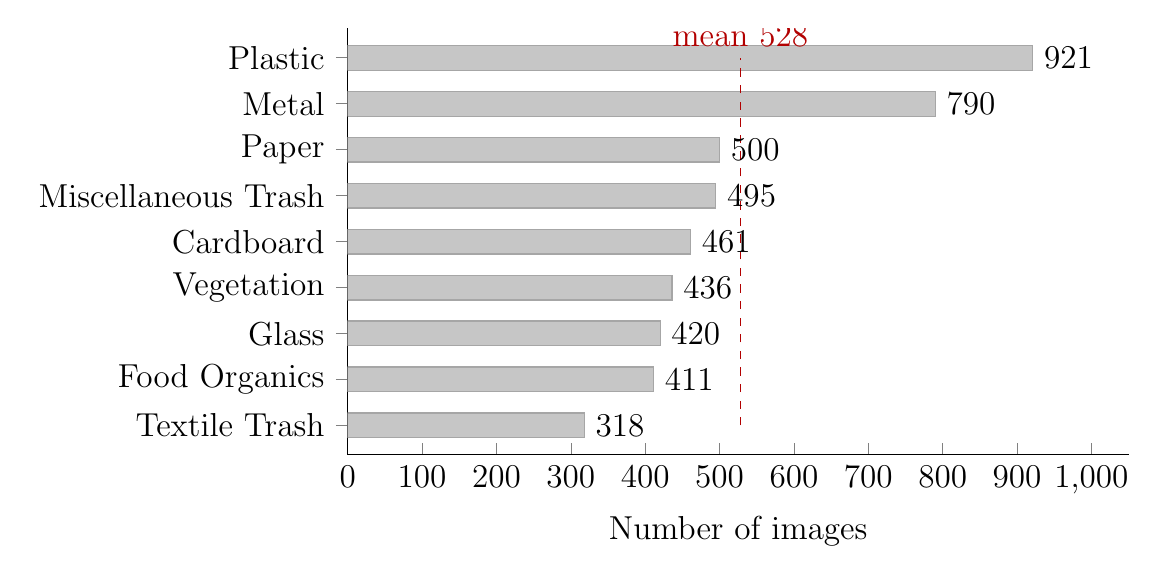
\begin{tikzpicture}
\begin{axis}[
  xbar, width=11.5cm, height=7cm, bar width=9pt,
  xmin=0, xmax=1050, xlabel={Number of images},
  symbolic y coords={Textile Trash,Food Organics,Glass,Vegetation,Cardboard,Miscellaneous Trash,Paper,Metal,Plastic},
  ytick=data, y tick label style={font=\small}, x tick label style={font=\small},
  nodes near coords, nodes near coords style={font=\small},
  axis x line*=bottom, axis y line*=left, enlarge y limits=0.08,
]
\addplot[fill=gray!45, draw=gray!70] coordinates {
  (318,Textile Trash) (411,Food Organics) (420,Glass) (436,Vegetation) (461,Cardboard)
  (495,Miscellaneous Trash) (500,Paper) (790,Metal) (921,Plastic)};
\draw[dashed, red!70!black] (axis cs:528,Textile Trash) -- (axis cs:528,Plastic)
  node[pos=1, above, font=\small, red!70!black] {mean 528};
\end{axis}
\end{tikzpicture}
\caption{Images per class in our copy of RealWaste (4,752 images). Plastic has 2.9 times as many images as Textile Trash.}
\label{fig:classes}
\end{figure}

When we looked through the images, the first thing we noticed was how uniform they are. Every photo shows one item from above on the same concrete floor, so the background tells the model nothing about the class. What does change is the lighting and colour cast: some photos are greyish, others clearly blue. A few items are hard even for a person. One ``Cardboard'' photo, for example, is printed food packaging that we would have labelled as Paper or Plastic. Figure~\ref{fig:samples} shows some examples.

\begin{figure}[H]
\centering
\figfile{sample_grid.png}{0.95\textwidth}{Drive: 04\_Results/dataset\_audit/sample\_grid.png}
\caption{Three sample images per class.}
\label{fig:samples}
\end{figure}

\section{III. CNN Model Design}

\subsection{1. Preprocessing}

\subsubsection{Cleaning and duplicate check}

There was little to clean in the usual sense: all 4,752 files opened without errors and no two files were byte-for-byte identical. The problem we did find was less obvious. To look for near-duplicates we computed a 256-bit difference hash of every image, a fingerprint that changes little when a photo is re-saved or slightly edited, and inspected the most similar pairs. That turned up only one near-identical pair across subsets. We then also looked at 32 random groups of three images with consecutive file numbers, and in 17 of them the same object had simply been photographed again, usually moved or turned over. The hash had missed these because the photos really are different. Under our first, random split, 4 of those 32 objects had one photo in the training set and another in validation or test, which means the test score would partly reward memorising objects.

\subsubsection{Grouped split}

Since re-shots almost always have neighbouring file numbers, we split by groups of numbers instead of by single images. Within each class, the files are cut into blocks of ten consecutive numbers (Plastic\_640 to Plastic\_649 form one block). The blocks are shuffled with seed 42, and whole blocks go to the training, validation or test set in a 70/15/15 ratio per class. Table~\ref{tab:leak} shows how much this reduced the leakage, and Table~\ref{tab:split} gives the final sizes.

\begin{table}[H]
\centering
\caption{Leakage checks for the random image-level split we started with and for the grouped split we used.}
\label{tab:leak}
\begin{tabularx}{\textwidth}{Xcc}
\toprule
Check & Random split & Grouped split \\
\midrule
Same-class pairs 1 file number apart, in different subsets & 46.7\,\% & 4.7\,\% \\
Same-class pairs 2 file numbers apart, in different subsets & 45.8\,\% & 9.4\,\% \\
Smallest hash distance, val/test image to nearest train image & 22 & 29 \\
Spot-check objects with photos in train and in val/test & 4 of 32 & 1 of 32 \\
\bottomrule
\end{tabularx}
\end{table}

\begin{table}[H]
\centering
\caption{Subsets of the grouped split (seed 42), shared by every model.}
\label{tab:split}
\begin{tabular}{lrrl}
\toprule
Subset & Images & Share & Purpose \\
\midrule
Training & 3,326 & 69.99\,\% & fit the weights \\
Validation & 719 & 15.13\,\% & early stopping and checkpoint selection \\
Test & 707 & 14.88\,\% & final evaluation, used once \\
\midrule
Total & 4,752 & 100\,\% & \\
\bottomrule
\end{tabular}
\end{table}

The split is not perfect. In the same 32 groups we still found one object, a heart-shaped ornament photographed front and back as Miscellaneous Trash 59 and 60, that falls on both sides of a block boundary. Re-shots that are far apart in numbering would also slip through. We come back to this in the limitations. To make sure every model saw exactly the same images, the split was saved once and its SHA-256 hash is checked each time it is loaded.

\subsubsection{Normalisation}

Images are converted to RGB, scaled to $[0,1]$ and normalised per channel with the ImageNet mean $(0.485, 0.456, 0.406)$ and standard deviation $(0.229, 0.224, 0.225)$. EfficientNet-B0 expects exactly these values. We used them for the two models trained from scratch as well, so that the only difference between the models is the model itself. Because the values are fixed constants, nothing is estimated from our own data, including the test set.

\subsubsection{Augmentation (training set only)}

\begin{table}[H]
\centering
\caption{Training augmentation, applied anew every epoch. Validation and test images are only resized to $224\times224$ and normalised.}
\label{tab:aug}
\begin{tabular}{ll}
\toprule
Step & Setting \\
\midrule
Random resized crop & 80 to 100\,\% of the image area, output $224\times224$ \\
Horizontal flip & probability 0.5 \\
Rotation & up to $\pm10^\circ$ \\
Colour jitter & brightness, contrast and saturation 0.2; hue unchanged \\
\bottomrule
\end{tabular}
\end{table}

The photos are square, so no cropping is needed at evaluation time. E1, E2 and E3 use the same augmentation. E4 uses none, since it exists only to measure what augmentation does.

\subsection{2. Simple CNN (E1)}

Our first model is meant as a baseline and is kept small on purpose. It has three convolution blocks, each made of a $3\times3$ convolution, batch normalisation, ReLU and $2\times2$ max pooling, followed by global average pooling and a small dense head (Figure~\ref{fig:e1}). The number of filters doubles from block to block (32, 64, 128) while the feature maps shrink from 224 to 28 pixels per side. In total the model has 111,145 parameters (Table~\ref{tab:e1}).

\begin{figure}[H]
\centering
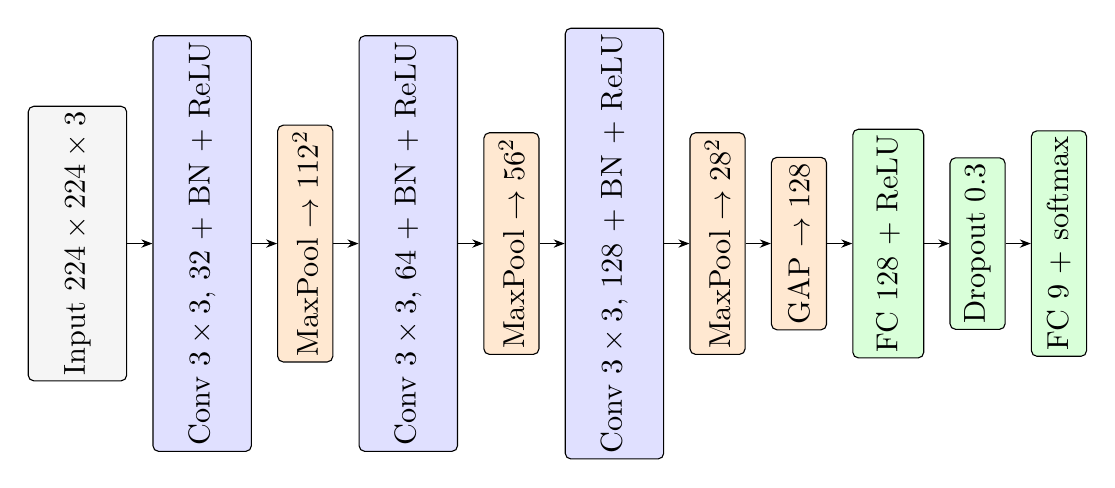
\begin{tikzpicture}[node distance=0.32cm]
  \node[plain, minimum height=3.0cm] (in) {\rotatebox{90}{Input $224\times224\times3$}};
  \node[conv, minimum height=2.6cm, right=of in] (c1) {\rotatebox{90}{Conv $3\times3$, 32 + BN + ReLU}};
  \node[pool, minimum height=2.6cm, right=of c1, minimum width=0.7cm] (p1) {\rotatebox{90}{MaxPool $\to 112^2$}};
  \node[conv, minimum height=2.2cm, right=of p1] (c2) {\rotatebox{90}{Conv $3\times3$, 64 + BN + ReLU}};
  \node[pool, minimum height=2.2cm, right=of c2, minimum width=0.7cm] (p2) {\rotatebox{90}{MaxPool $\to 56^2$}};
  \node[conv, minimum height=2.2cm, right=of p2] (c3) {\rotatebox{90}{Conv $3\times3$, 128 + BN + ReLU}};
  \node[pool, minimum height=2.2cm, right=of c3, minimum width=0.7cm] (p3) {\rotatebox{90}{MaxPool $\to 28^2$}};
  \node[pool, minimum height=1.6cm, right=of p3, minimum width=0.7cm] (gap) {\rotatebox{90}{GAP $\to 128$}};
  \node[dense, minimum height=1.6cm, right=of gap, minimum width=0.9cm] (f1) {\rotatebox{90}{FC 128 + ReLU}};
  \node[dense, minimum height=1.6cm, right=of f1, minimum width=0.7cm] (d) {\rotatebox{90}{Dropout 0.3}};
  \node[dense, minimum height=1.6cm, right=of d, minimum width=0.7cm] (f2) {\rotatebox{90}{FC 9 + softmax}};
  \foreach \a/\b in {in/c1, c1/p1, p1/c2, c2/p2, p2/c3, c3/p3, p3/gap, gap/f1, f1/d, d/f2} \draw[flow] (\a) -- (\b);
\end{tikzpicture}
\caption{Architecture of E1 SimpleCNN. Blue: convolution, orange: pooling, green: fully connected part.}
\label{fig:e1}
\end{figure}

\begin{table}[H]
\centering
\caption{E1 layers, output shapes and parameter counts.}
\label{tab:e1}
\begin{tabular}{lrr}
\toprule
Layer & Output shape & Parameters \\
\midrule
Input & $224\times224\times3$ & 0 \\
Conv $3\times3$ (32), BN, ReLU, MaxPool & $112\times112\times32$ & 928 \\
Conv $3\times3$ (64), BN, ReLU, MaxPool & $56\times56\times64$ & 18,560 \\
Conv $3\times3$ (128), BN, ReLU, MaxPool & $28\times28\times128$ & 73,984 \\
Global average pooling & 128 & 0 \\
Dense 128, ReLU, Dropout 0.3 & 128 & 16,512 \\
Dense 9 (logits) & 9 & 1,161 \\
\midrule
Total & & 111,145 \\
\bottomrule
\end{tabular}
\end{table}

The convolutions have no bias, since the batch normalisation right after them already adds one. A useful way to see the limits of this design is the receptive field: after three blocks, one value of the last feature map depends on a patch of only $22\times22$ input pixels. That is enough to recognise a texture but not the outline of a bottle or a box, so E1 should have trouble with classes that are recognised by their shape.

\subsection{3. Complex CNN: MultiScaleCNN (E2)}

For the complex model we started from a question raised in the lecture on modern CNNs: what is the right size for a convolution kernel? The lecture's answer, taken from GoogLeNet, is that combining several sizes can work better than picking one \cite{lec52, inception}. This fits our data. A crumpled plastic bag is recognised by fine wrinkles and reflections, which a small kernel picks up, while a cardboard box is recognised by large flat faces and straight edges. So each block of our network runs a $1\times1$, a $3\times3$ and a $5\times5$ convolution side by side on the same input and stacks their outputs (Figure~\ref{fig:msblock}). Half of the output channels go to the $3\times3$ branch and a quarter to each of the others. Compared with the Inception block in the lecture we left out the extra $1\times1$ reductions and the pooling branch to keep the model simple.

\begin{figure}[H]
\centering
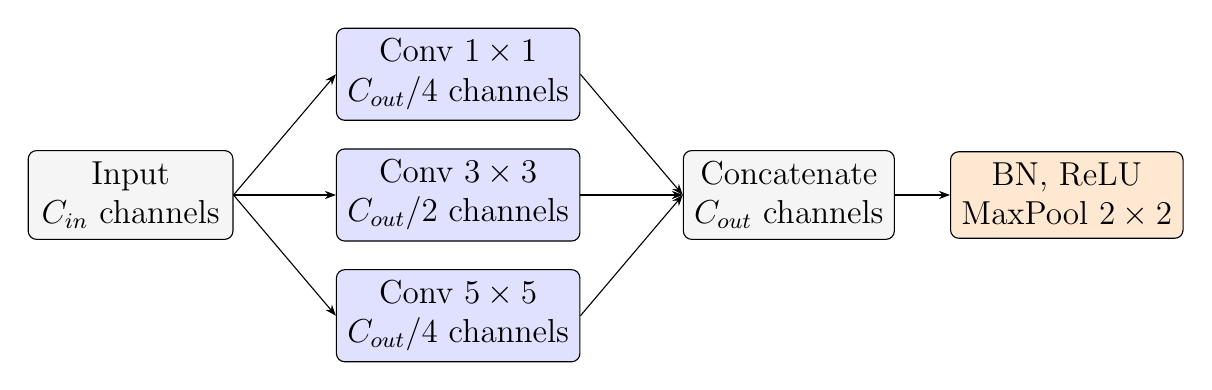
\begin{tikzpicture}[box/.style={draw, rounded corners=3pt, minimum width=2.6cm, minimum height=1.0cm, align=center, font=\small}]
  \node[box, fill=gray!8] (x) {Input\\ $C_{in}$ channels};
  \node[box, fill=blue!12, right=1.3cm of x] (b3) {Conv $3\times3$\\ $C_{out}/2$ channels};
  \node[box, fill=blue!12, above=0.35cm of b3] (b1) {Conv $1\times1$\\ $C_{out}/4$ channels};
  \node[box, fill=blue!12, below=0.35cm of b3] (b5) {Conv $5\times5$\\ $C_{out}/4$ channels};
  \node[box, fill=gray!8, right=1.3cm of b3] (cat) {Concatenate\\ $C_{out}$ channels};
  \node[box, fill=orange!18, right=0.7cm of cat] (out) {BN, ReLU\\ MaxPool $2\times2$};
  \foreach \b in {b1, b3, b5} {\draw[flow] (x.east) -- (\b.west); \draw[flow] (\b.east) -- (cat.west);}
  \draw[flow] (cat) -- (out);
\end{tikzpicture}
\caption{One multi-scale block. The three branches see the same input and are joined along the channel axis. Blocks 1 to 4 use $C_{out}$ = 64, 128, 256 and 256.}
\label{fig:msblock}
\end{figure}

The full network (Figure~\ref{fig:e2}) starts with a single $3\times3$ convolution as a stem, then has four multi-scale blocks, each followed by max pooling, and ends with the same kind of head as E1. It has 1,230,377 parameters, about eleven times more than E1 (Table~\ref{tab:e2}).

\begin{figure}[H]
\centering
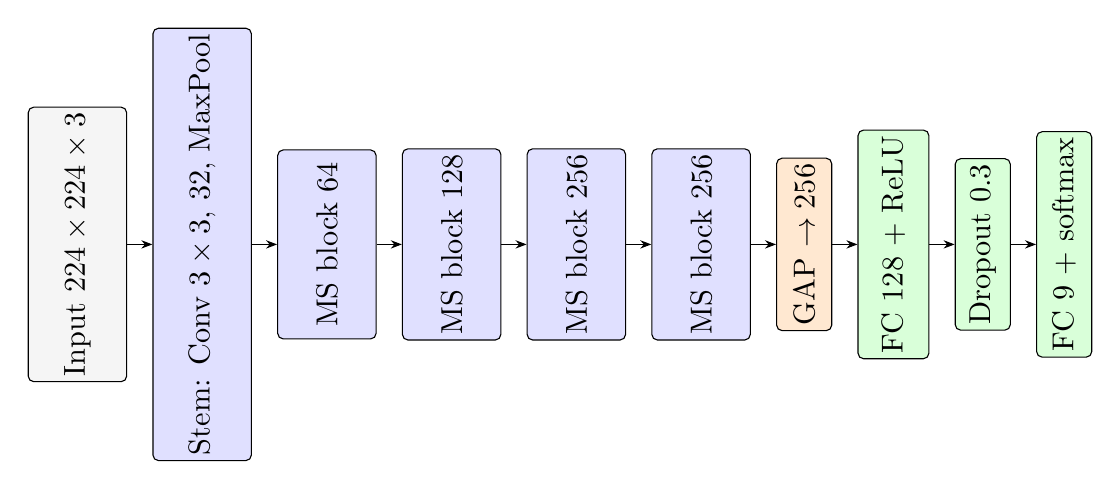
\begin{tikzpicture}[node distance=0.32cm]
  \node[plain, minimum height=3.0cm] (in) {\rotatebox{90}{Input $224\times224\times3$}};
  \node[conv, minimum height=2.7cm, right=of in] (s) {\rotatebox{90}{Stem: Conv $3\times3$, 32, MaxPool}};
  \node[conv, minimum height=2.4cm, right=of s] (m1) {\rotatebox{90}{MS block 64}};
  \node[conv, minimum height=2.1cm, right=of m1] (m2) {\rotatebox{90}{MS block 128}};
  \node[conv, minimum height=1.8cm, right=of m2] (m3) {\rotatebox{90}{MS block 256}};
  \node[conv, minimum height=1.8cm, right=of m3] (m4) {\rotatebox{90}{MS block 256}};
  \node[pool, minimum height=1.6cm, right=of m4, minimum width=0.7cm] (gap) {\rotatebox{90}{GAP $\to 256$}};
  \node[dense, minimum height=1.6cm, right=of gap, minimum width=0.9cm] (f1) {\rotatebox{90}{FC 128 + ReLU}};
  \node[dense, minimum height=1.6cm, right=of f1, minimum width=0.7cm] (d) {\rotatebox{90}{Dropout 0.3}};
  \node[dense, minimum height=1.6cm, right=of d, minimum width=0.7cm] (f2) {\rotatebox{90}{FC 9 + softmax}};
  \foreach \a/\b in {in/s, s/m1, m1/m2, m2/m3, m3/m4, m4/gap, gap/f1, f1/d, d/f2} \draw[flow] (\a) -- (\b);
\end{tikzpicture}
\caption{Architecture of E2 MultiScaleCNN. Every multi-scale (MS) block is followed by $2\times2$ max pooling, so the feature maps go from 112 to 7 pixels per side.}
\label{fig:e2}
\end{figure}

\begin{table}[H]
\centering
\caption{E2 stages. Channel counts in brackets are the $1\times1$ / $3\times3$ / $5\times5$ branches.}
\label{tab:e2}
\begin{tabular}{lrr}
\toprule
Stage & Output shape & Parameters \\
\midrule
Stem: Conv $3\times3$, 32, BN, ReLU, MaxPool & $112\times112\times32$ & 928 \\
MS block 1 (16 / 32 / 16), MaxPool & $56\times56\times64$ & 22,656 \\
MS block 2 (32 / 64 / 32), MaxPool & $28\times28\times128$ & 90,368 \\
MS block 3 (64 / 128 / 64), MaxPool & $14\times14\times256$ & 360,960 \\
MS block 4 (64 / 128 / 64), MaxPool & $7\times7\times256$ & 721,408 \\
Global average pooling & 256 & 0 \\
Dense 128, ReLU, Dropout 0.3 & 128 & 32,896 \\
Dense 9 (logits) & 9 & 1,161 \\
\midrule
Total & & 1,230,377 \\
\bottomrule
\end{tabular}
\end{table}

Through its $5\times5$ branches the last block of E2 sees a $154\times154$ pixel area of the input, against $22\times22$ for E1, so it can use the shape of the whole item. One caveat: E2 is not only multi-scale but also deeper and wider than E1. If E2 wins, we can only credit the design as a whole, not the multi-scale branches by themselves.

\subsection{4. Transfer Learning and Fine-Tuning: EfficientNet-B0 (E3)}

For transfer learning we chose EfficientNet-B0 \cite{efficientnet}, mainly because it is accurate for its size and trains quickly on the free Colab GPU we had. With its original 1,000-class head it has 5.3 million parameters and reaches 77.7\,\% top-1 accuracy on ImageNet-1K \cite{torchvision}. The network is built from MBConv blocks. Each block widens the channels with a $1\times1$ convolution, applies a cheap depthwise $3\times3$ or $5\times5$ convolution (one filter per channel), reweights the channels with a squeeze-and-excitation step and narrows them again with another $1\times1$ convolution. We removed the ImageNet head and put Dropout(0.2) and a $1280\to9$ dense layer in its place, which gives 4,019,077 parameters (Figure~\ref{fig:e3}).

\begin{figure}[H]
\centering
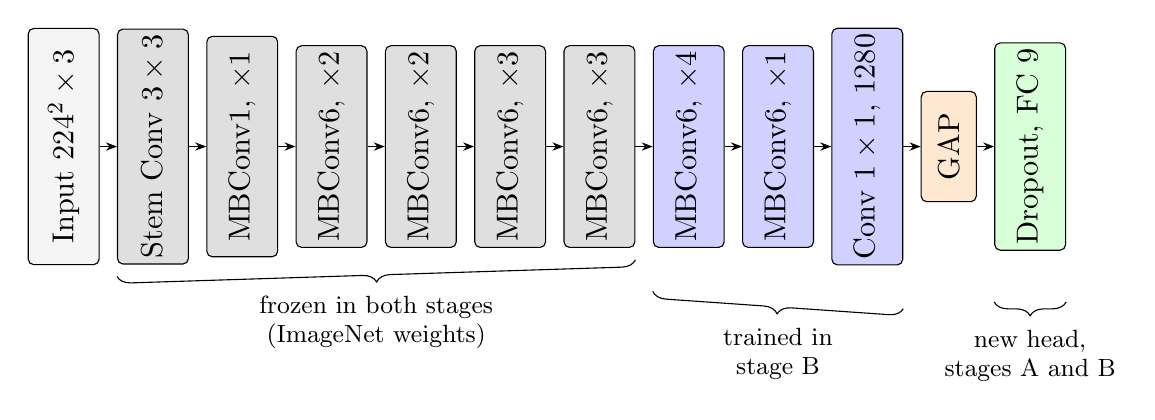
\begin{tikzpicture}[node distance=0.22cm]
  \node[plain, minimum height=3.0cm, minimum width=0.9cm] (in) {\rotatebox{90}{Input $224^2\times3$}};
  \node[frozen, minimum height=2.8cm, minimum width=0.9cm, right=of in] (f0) {\rotatebox{90}{Stem Conv $3\times3$}};
  \node[frozen, minimum height=2.8cm, minimum width=0.9cm, right=of f0] (f1) {\rotatebox{90}{MBConv1, $\times1$}};
  \node[frozen, minimum height=2.5cm, minimum width=0.9cm, right=of f1] (f2) {\rotatebox{90}{MBConv6, $\times2$}};
  \node[frozen, minimum height=2.2cm, minimum width=0.9cm, right=of f2] (f3) {\rotatebox{90}{MBConv6, $\times2$}};
  \node[frozen, minimum height=1.9cm, minimum width=0.9cm, right=of f3] (f4) {\rotatebox{90}{MBConv6, $\times3$}};
  \node[frozen, minimum height=1.9cm, minimum width=0.9cm, right=of f4] (f5) {\rotatebox{90}{MBConv6, $\times3$}};
  \node[tuned, minimum height=1.6cm, minimum width=0.9cm, right=of f5] (f6) {\rotatebox{90}{MBConv6, $\times4$}};
  \node[tuned, minimum height=1.6cm, minimum width=0.9cm, right=of f6] (f7) {\rotatebox{90}{MBConv6, $\times1$}};
  \node[tuned, minimum height=1.6cm, minimum width=0.9cm, right=of f7] (f8) {\rotatebox{90}{Conv $1\times1$, 1280}};
  \node[pool, minimum height=1.4cm, minimum width=0.7cm, right=of f8] (gap) {\rotatebox{90}{GAP}};
  \node[dense, minimum height=1.4cm, minimum width=0.9cm, right=of gap] (h) {\rotatebox{90}{Dropout, FC 9}};
  \foreach \a/\b in {in/f0, f0/f1, f1/f2, f2/f3, f3/f4, f4/f5, f5/f6, f6/f7, f7/f8, f8/gap, gap/h} \draw[flow] (\a) -- (\b);
  \draw[decorate, decoration={brace, mirror, amplitude=5pt}] ($(f0.south west)+(0,-0.15)$) -- ($(f5.south east)+(0,-0.15)$)
    node[midway, below=6pt, font=\scriptsize, align=center] {frozen in both stages\\ (ImageNet weights)};
  \draw[decorate, decoration={brace, mirror, amplitude=5pt}] ($(f6.south west)+(0,-0.55)$) -- ($(f8.south east)+(0,-0.55)$)
    node[midway, below=6pt, font=\scriptsize, align=center] {trained in\\ stage B};
  \draw[decorate, decoration={brace, mirror, amplitude=5pt}] ($(h.south west)+(0,-0.65)$) -- ($(h.south east)+(0,-0.65)$)
    node[midway, below=6pt, font=\scriptsize, align=center] {new head,\\ stages A and B};
\end{tikzpicture}
\caption{E3: EfficientNet-B0 with a new 9-class head. Grey blocks keep their ImageNet weights; the three blue blocks (\texttt{features[6:]}, all at $7\times7$ resolution) are fine-tuned in stage B.}
\label{fig:e3}
\end{figure}

Training happens in two stages that match the transfer and fine-tuning phases of the lecture \cite{lec53} (Table~\ref{tab:e3}). In stage A the whole backbone is frozen, including the running statistics of its batch normalisation layers, and only the new head learns. This is feature extraction: the backbone acts as a fixed feature generator and the head learns to read its 1,280 outputs. Stage B starts from the best stage-A checkpoint and also unfreezes the last three blocks, which hold the most task-specific features. We kept the first six blocks frozen because they detect generic edges and textures that should work for waste photos too, and because this keeps each epoch short. Whichever stage reaches the higher validation macro-F1 becomes the final E3 model.

\begin{table}[H]
\centering
\caption{The two training stages of E3.}
\label{tab:e3}
\begin{tabularx}{\textwidth}{lXX}
\toprule
 & Stage A: feature extraction & Stage B: fine-tuning \\
\midrule
Starts from & ImageNet weights, new random head & best stage-A checkpoint \\
Trainable part & head only & last 3 backbone blocks and head \\
Trainable parameters & 11,529 & 3,167,269 (79\,\%) \\
Learning rate (AdamW) & $10^{-3}$ & $10^{-4}$ \\
Maximum epochs & 10 & 15 \\
\bottomrule
\end{tabularx}
\end{table}

E3 is different from E1 and E2 in its pretrained weights, its architecture and its training schedule. Comparing them therefore tells us how transfer learning does against training from scratch, not which architecture is better.

\subsection{5. Training Protocol}

Table~\ref{tab:train} lists the training settings. We fixed them before training any model and used the same values for all models trained from scratch; E3 only differs where its two stages require it.

\begin{table}[H]
\centering
\caption{Training settings.}
\label{tab:train}
\begin{tabularx}{\textwidth}{lXX}
\toprule
Setting & E1, E2, E4 & E3 \\
\midrule
Loss & cross-entropy, no class weights & same \\
Optimiser & AdamW, lr $10^{-3}$, weight decay $10^{-4}$ & AdamW, lr $10^{-3}$ (stage A) and $10^{-4}$ (stage B), weight decay $10^{-4}$ \\
Learning-rate schedule & halved after 2 epochs without a better validation macro-F1 & same, per stage \\
Batch size & 32 & 32 \\
Maximum epochs & 40 & 10 + 15 \\
Early stopping & 5 epochs without a better validation macro-F1 & same, per stage \\
Checkpoint kept & best validation macro-F1 & best of both stages \\
Precision & mixed (16-bit) on GPU & same \\
\bottomrule
\end{tabularx}
\end{table}

A few of these choices came out of the project itself. We first gave E1 a limit of 30 epochs, but its validation score was still rising at epoch 30, so we raised the limit to 40 for both models trained from scratch and let the same run continue. We also considered weighting the loss by class frequency. We decided against it after E2 had been trained, because the deeper model already recovered most of the small classes on its own (validation recall for Textile Trash went from 29\,\% with E1 to 51\,\% with E2, and for Miscellaneous Trash from 30\,\% to 70\,\%).

We select models by validation macro-F1 rather than accuracy, both for early stopping and for picking the epoch to keep. With unequal classes, macro-F1 gives Textile Trash the same weight as Plastic.

We did not run a hyperparameter search. We had planned a small one (two learning rates and then two values of one more setting for each model), but it did not fit into the deadline. The values in Table~\ref{tab:train} are common defaults for AdamW and for fine-tuning. They may not be the best for every model, E1 in particular.

What we did instead was to repeat training. A single run depends on chance: the starting weights, the order of the batches, which augmentations are drawn and which neurons dropout switches off. So E1, E2 and E3 were each trained three times, with seeds 42, 43 and 44, and we report the mean and standard deviation (SD). The split stays the same in all runs, so the SD shows how much the result moves with training randomness, not with the choice of test images. E4 was trained once.

All training ran on Google Colab with an NVIDIA T4 GPU, about 40 seconds per epoch for E1 and E3 and 45 seconds for E2. In practice the slowest part was reading the images from Google Drive: the first epoch of a new session took around 15 minutes, until we started copying the dataset to the Colab disk at the beginning of each session.

% ------------------------------------------------------------------ IV
\section{IV. Experimental Results}

\subsection{1. Metrics}

We report accuracy and the macro averages of precision, recall and F1. For a class $k$, precision $P_k$ is the share of images predicted as $k$ that really belong to $k$, and recall $R_k$ is the share of the real $k$ images that the model found. F1 combines the two, and the macro average gives every class the same weight:
\begin{equation}
  F1_k = \frac{2\,P_k R_k}{P_k + R_k}, \qquad \text{Macro-F1} = \frac{1}{K}\sum_{k=1}^{K} F1_k .
\end{equation}
Macro precision and macro recall are averaged in the same way. Accuracy, the share of all images classified correctly, is easier to read but can hide a weak small class, which is why we use macro-F1 to compare models.

\subsection{2. Results on the Test Set}

\todo{fill Table~\ref{tab:test} from \texttt{04\_Results/final/model\_comparison.csv} after notebook 09 has run with all three seeds, then delete this note.}

\begin{table}[H]
\centering
\caption{Test set (707 images). E1 to E3: mean $\pm$ SD over seeds 42, 43 and 44. E4: one run. Precision, recall and F1 are macro averages.}
\label{tab:test}
\begin{tabular}{lcccc}
\toprule
Model & Accuracy & Precision & Recall & F1-score \\
\midrule
E1 SimpleCNN & \tbd & \tbd & \tbd & \tbd \\
E2 MultiScaleCNN & \tbd & \tbd & \tbd & \tbd \\
E3 EfficientNet-B0 (fine-tuned) & \tbd & \tbd & \tbd & \tbd \\
E4 MultiScaleCNN, no augmentation & \tbd & \tbd & \tbd & \tbd \\
\bottomrule
\end{tabular}
\end{table}

\todo{per-class test F1 from \texttt{04\_Results/final/per\_class\_f1.csv}, one sentence on the hardest classes.}

\begin{figure}[H]
\centering
\figfile{E1_confusion_matrix.png}{0.48\textwidth}{Drive: 04\_Results/experiments/E1/}\hfill
\figfile{E2_confusion_matrix.png}{0.48\textwidth}{Drive: 04\_Results/experiments/E2/}\\[6pt]
\figfile{E3_confusion_matrix.png}{0.48\textwidth}{Drive: 04\_Results/experiments/E3/}\hfill
\figfile{E4_confusion_matrix.png}{0.48\textwidth}{Drive: 04\_Results/experiments/E4/}
\caption{Test confusion matrices of the seed-42 runs (rows: true class, columns: predicted class).}
\label{fig:cm}
\end{figure}

\subsection{3. Validation Results and Training Behaviour}

Table~\ref{tab:val} shows the validation scores of the seed-42 runs, the scores we used to pick each checkpoint. On the 719 validation images the ranking was clear: E1 reached a macro-F1 of 0.650, E2 0.787 and E3 0.879, so each step up added roughly 0.1.

\begin{table}[H]
\centering
\caption{Validation set (719 images), seed-42 runs, selected checkpoints.}
\label{tab:val}
\begin{tabular}{lccccc}
\toprule
Model & Best epoch & Accuracy & Precision & Recall & F1-score \\
\midrule
E1 SimpleCNN & 33 of 38 & 0.656 & 0.706 & 0.636 & 0.650 \\
E2 MultiScaleCNN & 35 of 40 & 0.787 & 0.815 & 0.772 & 0.787 \\
E3 EfficientNet-B0 & 25 of 25 & 0.880 & 0.894 & 0.871 & 0.879 \\
E4 no augmentation & 29 of 34 & 0.814 & 0.819 & 0.803 & 0.808 \\
\bottomrule
\end{tabular}
\end{table}

\todo{add the validation macro-F1 mean $\pm$ SD of the three seeds from each \texttt{selection.json}.}

The training curves (Figure~\ref{fig:curves}) explain part of this ranking. E1 kept improving slowly until about epoch 33, and its training and validation curves stayed close the whole time. It was not overfitting, it simply did not have enough capacity. E2 behaved differently: after roughly epoch 30 its training loss kept going down (0.49 at the end) while the validation loss stayed around 0.64, a mild overfit that is harmless because we keep the best validation epoch anyway. E3 was the most interesting case. With only the head trained, stage A already reached 0.810, better than our best model trained from scratch. Fine-tuning in stage B raised this to 0.879, but by the end of stage B the training accuracy was close to 100\,\% (training loss 0.02 against 0.42 on validation), so we saw no point in training it longer.

\begin{figure}[H]
\centering
\figfile{E1_curves.png}{0.95\textwidth}{Drive: 04\_Results/experiments/E1/}\\[4pt]
\figfile{E2_curves.png}{0.95\textwidth}{Drive: 04\_Results/experiments/E2/}\\[4pt]
\figfile{E3_curves.png}{0.95\textwidth}{Drive: 04\_Results/experiments/E3/}
\caption{Training and validation loss, accuracy and macro-F1 per epoch for E1, E2 and E3 (seed 42).}
\label{fig:curves}
\end{figure}

\subsection{4. Augmentation Ablation (RQ4)}

The ablation result goes against the usual expectation. Without augmentation, the multi-scale CNN (E4) reached 0.808 validation macro-F1, slightly more than the 0.787 of the same model with augmentation (E2). We do not think this shows that augmentation hurts. The gap is 0.021 from a single run of each model, and the validation macro-F1 of one model often moved by up to 0.04 from one epoch to the next. The loss curves tell a clearer story: without augmentation the training loss fell to about 0.22 while the validation loss stayed near 0.57, whereas with augmentation the two stayed much closer (0.49 and 0.64). Augmentation clearly regularised the model; it just did not turn this into a better score within 40 epochs.

We can think of three reasons, none of which we tested. The photos are already very uniform (same camera angle, same floor, centred objects), so random crops and rotations add variety that the test images do not have. Colour jitter may blur colour differences that matter for classes such as Cardboard or Vegetation. And augmented training usually needs more epochs than we gave it. \todo{compare E2 and E4 on the test set, keeping in mind that E4 has one run.}

\subsection{5. Error Analysis}

Looking at the validation errors, one pattern stood out for every model: when unsure, the models tended to answer ``Plastic''. For E1 this was extreme. It predicted Plastic for 249 validation images, of which only 116 really were Plastic, so 54\,\% of all its errors were wrong Plastic predictions. The share dropped to 33\,\% for E2 and 31\,\% for E3. Plastic is the largest class and includes almost every shape, colour and degree of shine, which probably makes it the safest guess for a model that has not learned the other classes well. Table~\ref{tab:conf} lists the most common confusions.

\begin{table}[H]
\centering
\caption{Most frequent confusions on validation (true $\to$ predicted, number of images).}
\label{tab:conf}
\begin{tabularx}{\textwidth}{lX}
\toprule
Model & Confusions \\
\midrule
E1 & Metal $\to$ Plastic 34, Miscellaneous $\to$ Plastic 31, Glass $\to$ Plastic 25, Cardboard $\to$ Plastic 18 \\
E2 & Plastic $\to$ Metal 23, Cardboard $\to$ Plastic 17, Glass $\to$ Plastic 14, Textile $\to$ Miscellaneous 13 \\
E3 & Miscellaneous $\to$ Plastic 9, Glass $\to$ Plastic 8, Metal $\to$ Plastic 6, Cardboard $\to$ Metal 5 \\
\bottomrule
\end{tabularx}
\end{table}

The two hardest classes were Miscellaneous Trash and Textile Trash. E1 found only 30\,\% and 29\,\% of them. E2 found 70\,\% and 51\,\%, and E3 71\,\% and 82\,\%. Both classes are collections of very different objects rather than one material, and Textile Trash is also the smallest class, so these numbers are not surprising.

\todo{test error analysis: take the model with the best mean validation macro-F1, open its \texttt{errors.csv}, describe the failure modes of 50 to 100 misclassified test images grouped by confusion pair, and add a figure with example errors.}

% ------------------------------------------------------------------ V
\section{V. Conclusion}

\todo{the findings below come from validation. Replace each number with the test mean $\pm$ SD and keep a finding only if the test results still support it.}

The fine-tuned EfficientNet-B0 (E3) was clearly our best model, with a validation macro-F1 of 0.879, compared with 0.787 for our multi-scale CNN (E2) and 0.650 for the simple CNN (E1). Going back to the research questions:

\textbf{RQ1.} A three-block CNN trained from scratch reaches a macro-F1 of 0.650. It does not overfit, yet it misses most Textile Trash and Miscellaneous Trash items, which suggests that it is too small for the task rather than short of data.

\textbf{RQ2.} The multi-scale CNN improves macro-F1 by 0.137 and recovers much of the two hard classes. As E2 is also deeper and wider than E1, we credit this gain to the design as a whole.

\textbf{RQ3.} ImageNet pretraining adds about 0.09 macro-F1 on top of E2. The most telling result is that the frozen pretrained features with only a new head (0.810) already beat both models trained from scratch.

\textbf{RQ4.} Removing augmentation changed validation macro-F1 by $+0.021$, which is within the noise of a single run. Augmentation did narrow the gap between training and validation loss, but our experiment cannot show that it changes accuracy.

The errors that remain are mostly confusions between materials that look alike (glass, metal and plastic; cardboard and plastic), Plastic used as a fallback answer, and the two mixed classes.

The study has clear limitations. Photos of one object can still end up in different subsets when they straddle a block boundary or are far apart in numbering, so the test scores may be a little optimistic. We did not search for better hyperparameters, and E1 in particular might do better with other settings. The SD over three seeds only covers training randomness: all runs share one split, and E4 was run only once. Our comparisons also change more than one thing at a time, since E2 differs from E1 in several ways and E3 differs from both in pretraining and schedule. Last, all images come from one setup with the same floor and camera angle, and we expect lower accuracy on photos taken elsewhere, for example on a real sorting line.

For a practical system with a small labelled dataset, our results point towards starting from a pretrained network rather than designing a CNN from scratch: in our tests it was the most accurate model and needed only 25 epochs. Before using it in the field, though, it would have to be trained and tested on images from the place where it will run.

% ------------------------------------------------------------------ references
\begin{thebibliography}{99}
\setlength{\itemsep}{2pt}
\bibitem{lec51} N. T. K. Ngan, ``Convolutional Neural Network (CNN),'' lecture slides, Chapter 5.1, Deep Learning course, National Economics University, 2026.
\bibitem{lec52} N. T. K. Ngan, ``Modern Convolutional Neural Networks,'' lecture slides, Chapter 5.2, Deep Learning course, National Economics University, 2026.
\bibitem{lec53} N. T. K. Ngan, ``CNN Techniques,'' lecture slides, Chapter 5.3, Deep Learning course, National Economics University, 2026.
\bibitem{realwaste} S. Single, S. Iranmanesh, and R. Raad, ``RealWaste: A novel real-life data set for landfill waste classification using deep learning,'' \emph{Information}, vol.~14, no.~12, art.~633, 2023. \url{https://www.mdpi.com/2078-2489/14/12/633}. Dataset: UCI Machine Learning Repository, \url{https://archive.ics.uci.edu/dataset/908/realwaste}.
\bibitem{efficientnet} M. Tan and Q. V. Le, ``EfficientNet: Rethinking model scaling for convolutional neural networks,'' in \emph{Proc. ICML}, 2019. arXiv:1905.11946.
\bibitem{inception} C. Szegedy, W. Liu, Y. Jia, P. Sermanet, S. Reed, D. Anguelov, D. Erhan, V. Vanhoucke, and A. Rabinovich, ``Going deeper with convolutions,'' arXiv:1409.4842, 2014.
\bibitem{batchnorm} S. Ioffe and C. Szegedy, ``Batch normalization: Accelerating deep network training by reducing internal covariate shift,'' arXiv:1502.03167, 2015.
\bibitem{dropout} N. Srivastava, G. Hinton, A. Krizhevsky, I. Sutskever, and R. Salakhutdinov, ``Dropout: A simple way to prevent neural networks from overfitting,'' \emph{Journal of Machine Learning Research}, vol.~15, no.~56, pp.~1929--1958, 2014.
\bibitem{adamw} I. Loshchilov and F. Hutter, ``Decoupled weight decay regularization,'' in \emph{Proc. ICLR}, 2019. arXiv:1711.05101.
\bibitem{imagenet} O. Russakovsky, J. Deng, H. Su, et al., ``ImageNet large scale visual recognition challenge,'' arXiv:1409.0575, 2014.
\bibitem{torchvision} PyTorch, ``torchvision \texttt{efficientnet\_b0}, weights \texttt{IMAGENET1K\_V1},'' model documentation. \url{https://docs.pytorch.org/vision/main/models/generated/torchvision.models.efficientnet_b0.html}.
\end{thebibliography}

\end{document}
